\documentclass{article}
\usepackage{amsmath}
\usepackage{graphicx}
\usepackage[colorlinks=true, linkcolor=black, citecolor=cyan, urlcolor=darkgray]{hyperref}
\usepackage{dirtree}
\usepackage{tikz}
\usetikzlibrary{automata, positioning, arrows}

\usepackage{xepersian}
\settextfont{B Nazanin}

\newcommand{\english}[1]{\settextfont{Times New Roman} \lr{#1} \settextfont{B Nazanin}}

\title{تشخیص عواطف توسط دستگاه‌های پوشیدنی}
\begin{document}
	\maketitle
	\newpage
	\begin{abstract}
		تشخیص عواطف
	\end{abstract}
	\newpage
	\tableofcontents
	
	\section{عواطف}
	
	\section{مجموعه داده}
	مجموعه داده \english{WESAD\cite{wesad}} یکی از کامل‌ترین ﻣﺠﻤﻮﻋﻪ ﻫﺎﻱ ﺩﺍﺩﻩ ﺑﺮﺍﻱ ﺗﺸﺨﻴﺺ ﻋﻮﺍﻃﻒ ﺍﺳﺖ. ﺑﻴﺸﺘﺮﻳﻦ ﺗﻤﺮﻛﺰ ﻭ ﺍﺳﺘﻔﺎﺩﻩ ﺍﺯ ﺍﻳﻦ ﻣﺠﻤﻮﻋﻪ ﺑﺮﺍﻱ ﺗﺸﺨﻴﺺ ﺍﺳﺘﺮﺱ ﺑﻮﺩﻩﺍﺳﺖ. ﺑﺎ ﺍﻳﻦ ﻭﺟﻮﺩ، ﺑﻪ ﺟﺰ ﻛﻼﺱ ﺍﺳﺘﺮﺱ ﻭ ﻋﺎﺩﻱ، ﺑﺮﺍﻱ ﻧﺸﺨﻴﺺ ﻛﻼﺱ ﻫﺎﻱ ﺧﻮﺷﺤﺎﻟﻲ ﻭ ﺁﺭﺍﻣﺶ ﻧﻴﺰ ﻣﻲﺗﻮﺍﻥ ﺍﺯ ﺍﻳﻦ ﺩﺍﺩﻩﻫﺎ ﺍﺳﺘﻔﺎﺩﻩ ﻧﻤﻮﺩ. ﻋﻼﻭﻩ ﺑﺮ ﺁﻥﻫﺎ، ﻫﺮ ﺷﺨﺺ پﺮﺳﺸﻨﺎﻣﻪﻫﺎﻳﻲ ﻧﻴﺰ پﺮ ﻛﺮﺩﻩ ﻛﻪ ﺍﻳﻦ ﻫﻢ ﻣﻲﺗﻮﺍﻧﺪ ﺑﺎﻋﺚ ﺧﻠﻖ ﻣﺪﻝ ﻫﺎﻱ ﺟﺪﻳﺪﻱ ﺷﻮﺩ. ﺩﻭ ﺩﺳﺘگﺎﻩ ﺍﺻﻠﻲ ﺑﺮﺍﻱ ﻓﺮﺍﻫﻢ ﺁﻭﺭﺩﻥ ﺍﻳﻦ ﺩﺍﺩﻩﻫﺎ ﻣﻮﺭﺩ ﺍﺳﺘﻔﺎﺩﻩ ﻗﺮﺍﺭ گﺮﻓﺘﻪ ﺍﻧﺪ: \textbf{1(} مچ‌بند \english{Emaptica E4} ﻪ ﺑﺴﻴﺎﺭﻱ ﺍﺯ ﺩﺍﻧﺸگﺎﻩﻫﺎﻱ ﺳﺮﺍﺳﺮ ﺩﻧﻴﺎ ﺍﺯ ﺁﻥ ﺍﺳﺘﻔﺎﺩﻩ ﻣﻲ ﻛﻨﻨﺪ\cite{empatica} و  \textbf{2(} دستگاه \english{Repiban} که یکی از پیشرفته ترین سنسورهای تحقیقاتی است که بر روی سینه نصب می‌شود\cite{respiban}.
	
	\begin{figure}
		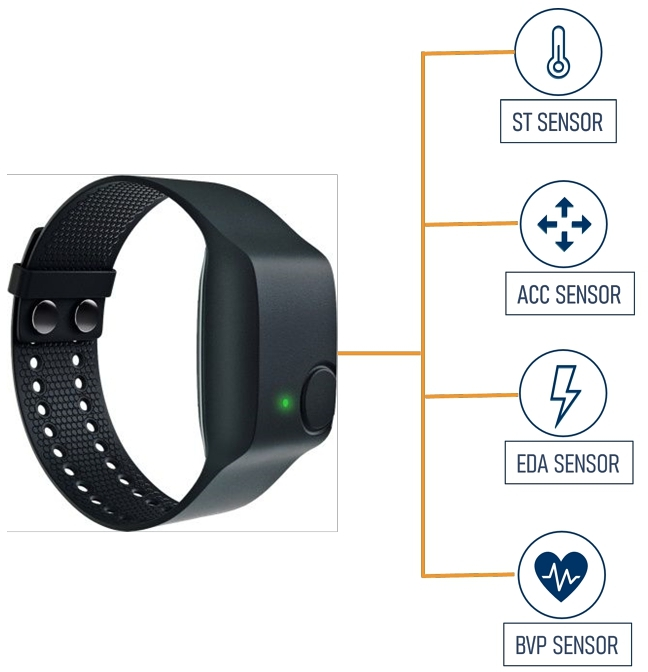
\includegraphics[width=0.5\textwidth]{empatica.jpg}
		\hspace{1cm}
		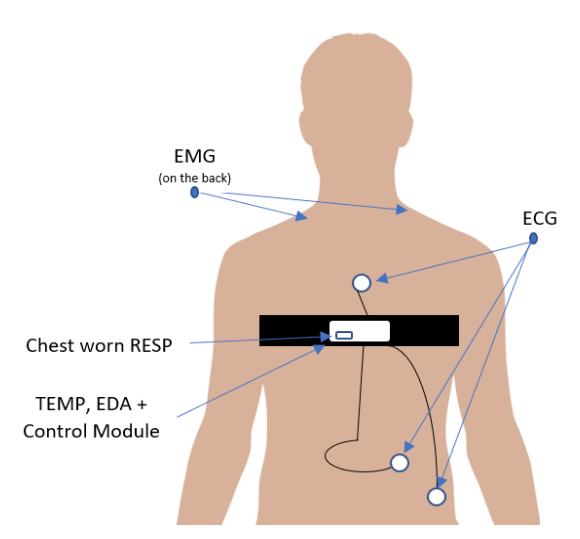
\includegraphics[width=0.5\textwidth]{respiban.png}
		\caption{شکل راست: ساعت \english{Empatica E4} ﺭﺍ ﻧﺸﺎﻥ ﻣﻲﺩﻫﺪ. ﺍﻳﻦ ﺳﺎﻋﺖ ﺑﻪ ﺩﻟﻴﻞ ﺳﻨﺴﻮﺭﻫﺎﻱ ﻛﺎﻣﻞ، ﺯﻳﺒﺎﻳﻲ ﻭ ﺭﺍﺣﺘﻲ ﺍﺳﺘﻔﺎﺩﻩ ﻛﺎﺭﺑﺮﺩ ﺯﻳﺎﺩﻱ ﺩﺭ ﺗﺤﻘﻴﻘﺎﺕ ﺩﺍﺭﺩ. 
		شکل چپ:‌ دستگاه \english{Respiban} ﻭ ﻧﺤﻮﻩ ﻗﺮﺍﺭگﻴﺮﻱ ﺁﻥ ﺭﻭﻱ ﺳﻴﻨﻪ ﻭ ﻣﺤﻞ ﻫﺮ ﻳﻚ ﺍﺯ ﺳﻨﺴﻮﺭﻫﺎ ﺭﺍ ﻧﺸﺎﻥ ﻣﻲ ﺩﻫﺪ.}
	\end{figure}
	\subsection{دستگاه \english{Respiban}}
	ﺍﻳﻦ ﺩﺳﺘگﺎﻩ ﻣﻲﺗﻮﺍﻧﺪ ۶ ﻋﺎﻣﻞ ﺭﺍ ﺍﻧﺪﺍﺯﻩگﻴﺮﻱ ﻛﻨﺪ. ﻓﺮﻛﺎﻧﺲ ﻭﺭﻭﺩﻱ ﺍﻳﻦ ﺩﺳﺘگﺎﻩ ﺑﺮﺍﻱ ﻫﻤﻪ ﺳﻨﺴﻮﺭﻫﺎﻳﺶ ۷۰۰ ﻫﺮﺗﺰ ﻣﻲﺑﺎﺷﺪ. ﺳﻨﺴﻮﺭﻫﺎﻱ ﺁﻥ ﺑﻪ ﺷﺮﺡ ﺯﻳﺮ ﺍﺳﺖ:
	\begin{enumerate}
		\item مختصات‌یابی (\english{Accelerometer})
		\item نوار قلب (\english{Electrocardiogram})
		\item فعالیت الکتریکی پوست (\english{Electrodermal Activity})
		\item برق‌ماهیچه‌نگار (\english{Electromyogram})
		\item تنفس (\english{Respiration})
		\item دما (\english{Temperature})
	\end{enumerate}
	
	\subsection{ساعت \english{Empatica E4}}
	ﺍﻳﻦ ﺳﺎﻋﺖ ﺷﺎﻣﻞ ﺳﻨﺴﻮﺭ ﻫﺎﻱ ﻣﺨﺘﺼﺎﺕ ﻳﺎﺑﻲ، فشار خون\footnote{\english{Blood Volume Pressure}}، دما . فعالیت الکتریکی پوست است. هر یک از این ﺳﻨﺴﻮﺭﻫﺎ ﺑﺎ ﻓﺮﻛﺎﻧﺲ ﻣﺘﻔﺎﻭﺗﻲ ﺍﻧﺪﺍﺯﻩگﻴﺮﻱ ﺷﺪﻩﺍﻧﺪ. ﺩﺭ ﺟﺪﻭﻝ ﻣﻘﺪﺍﺭ ﻓﺮﻛﺎﻧﺲ ﻫﺮ ﻳﻚ ﺍﺯ ﺳﻨﺴﻮﺭﻫﺎ ﺁﻭﺭﺩﻩ ﺷﺪﻩ ﺍﺳﺖ.
	
	\begin{table}[h]
		\begin{tabular}{|c|c|}
			\hline
			سنسور & فرکانس \\
			\hline
			\english{ACC} & 32\\
			\english{BVP} & 64\\
			\english{EDA} & 4\\
			\english{Temp} & 4\\
			\hline
		\end{tabular}
	\end{table}
	\subsection{پرسشنامه‌ها}
	ﻋﻼﻭﻩ ﺑﺮ ﺩﻭ ﺩﺳﺘگﺎﻩ گﻔﺘﻪ ﺷﺪﻩ، ﻫﺮ ﻳﻚ ﺍﺯ ﺳﻮژﻩﻫﺎﻱ ﺁﺯﻣﺎﻳﺶ، پﺮﺳﺸﻨﺎﻣﻪ ﻫﺎﻳﻲ ﺭﺍ پﺮ ﻛﺮﺩﻧﺪ. ﺍﻳﻦ پﺮﺳﺸﻨﺎﻣﻪﻫﺎ ﺩﺭ ﺟﻬﺖ ﺩﺭﻳﺎﻓﺖ ﺍﻃﻼﻋﺎﺕ ﺑﻴﺸﺘﺮ ﺩﺭ ﻣﻮﺭﺩ ﺍﺣﺴﺎﺳﺎﺕ ﺍﺷﺨﺎﺹ ﺑﻪ ﻛﺎﺭ گﺮﻓﺘﻪ ﺷﺪﻧﺪ، ﺍگﺮچﻪ ﺩﺭ ﻫﻴچﻳﻚ ﺍﺯ ﻣﻘﺎﻻﺕ ﺑﺮﺭﺳﻲ ﺷﺪﻩ،ﻣﺤﻘﻘﺎﻥ ﺍﺯ ﺍﻳﻦ پﺮﺳﺸﻨﺎﻣﻪ ﻫﺎ ﺍﺳﺘﻔﺎﺩﻩ ﺍﻱ ﻧﻜﺮﺩﻧﺪ. ﺩﺭ ﻗﺴﻤﺖﻫﺎﻱ پﻴﺶﺭﻭ ﺍﻳﻦ پﺮﺳﺸﻨﺎﻣﻪﻫﺎ ﺭﺍ ﺑﺮﺭﺳﻲ ﻣﻲ ﻛﻨﻴﻢ:
	
	\subsubsection*{\english{PANAS}}
	ﺳﻮژﻩ ﻣﻲﺑﺎﻳﺴﺖ ﺑﻪ ۲۶ ﺣﺲ ﺩﺭ پﺮﺳﺸﻨﺎﻣﻪ، ﺍﺯ ۱ ﺗﺎ ۵ ﺍﻣﺘﻴﺎﺯ ﺩﻫﺪ. ﺍﻳﻦ ﺍﺣﺴﺎﺳﺎﺕ ﻋﺒﺎﺭﺗﻨﺪ ﺍﺯ: ﻓﻌﺎﻝ، پﺮﻳﺸﺎﻧﻲ، ﻋﻼﻗﻪ ﻣﻨﺪ، ﺍﻟﻬﺎﻡﺷﺪﻩ، ﺭﻧﺠﻴﺪﻩ، گﻨﺎﻫﻜﺎﺭ، ﺗﺮﺳﻴﺪﻩ، ﺩﺷﻤﻨﻲ، ﻫﻴﺠﺎﻥﺯﺩﻩ، ﻣﻐﺮﻭﺭ، ﻛﺞﺧﻠﻖ، ﻣﺸﺘﺎﻕ، ﺷﺮﻣﻨﺪﻩ، ﻫﻮﺷﻴﺎﺭ، ﻧگﺮﺍﻥ، ﻣﺼﻤﻢ، ﻣﺘﻮﺟﻪ، ﻋﺼﺒﻲ، ﻭﺣﺸﺖﺯﺩﻩ، ﺍﺳﺘﺮﺳﻲ، ﺧﺴﺘﻪ، ﺧﻮﺷﺤﺎﻝ، ﻋﺼﺒﺎﻧﻲ، ﺁﺯﺭﺩﻩﺷﺪﻥ ﻭ ﻧﺎﺭﺍﺣﺖ.
	\subsubsection*{\english{STAI}}
	ﺩﺭ ﺍﻳﻦ پﺮﺳﺸﻨﺎﻣﻪ، ﺳﻮژﻩ ﺑﻪ ﻫﺮ ﻳﻚ ﺍﺯ ﺳﻮﺍﻝ ﻫﺎﻱ ﺯﻳﺮ ﺍﺯ ۱ ﺗﺎ ۴ ﻧﻤﺮﻩ ﻣﻲ ﺩﻫﺪ:
	\begin{enumerate}
		\item ﻣﻦ ﺍﺣﺴﺎﺱ ﺭﺍﺣﺘﻲ ﻣﻲ ﻛﻨﻢ
		\item ﻣﻦ ﺍﺣﺴﺎﺱ ﻧگﺮﺍﻧﻲ ﻣﻲ ﻛﻨﻢ
		\item ﻣﻦ ﻋﺼﺒﻲ ﻫﺴﺘﻢ
		\item ﻣﻦ ﺭﻳﻠﻜﺲ ﻫﺴﺘﻢ
		\item ﻣﻦ ﺍﺣﺴﺎﺱ ﺩﻟﻮﺍپﺴﻲ ﻣﻲ ﻛﻨﻢ
		\item ﻣﻦ ﺍﺣﺴﺎﺱ ﺭﺿﺎﻳﺖ ﻣﻲ ﻛﻨﻢ
	\end{enumerate}
	\subsubsection*{\english{SAM}}
	ﺍﻳﻦ ﺗﺴﺖ ﺷﺪﺕ ﻭ ﺧﻮﺏ ﻳﺎ ﺑﺪ ﺑﻮﺩﻥ ﺍﺣﺴﺎﺳﺎﺕ ﺭﺍ ﻣﻲ ﺳﻨﺠﺪ. ﺷﺨﺺ ﺩﻭ ﺳﻮﺍﻝ ﺭﺍ ﺩﺭ ﻣﻘﻴﺎﺱ ۱ ﺗﺎ ۹ پﺎﺳﺦ ﻣﻲ ﺩﻫﺪ: \textbf{1(} ﺣﺲ ﻣﻦ چقدر ﺧﻮﺏ ﺍﺳﺖ ﻭ \textbf{2(} ﺷﺪﺕ ﺍﻳﻦ ﺣﺲ چقدر ﺍﺳﺖ.
	\subsubsection*{\english{SSSQ}}
	ﺍﻳﻦ ﺗﺴﺖ ﻛﻪ ﻛﻮﺗﺎﻩﺷﺪﻩ ﺗﺴﺖ ﺍﺳﺘﺎﻧﺪﺍﺭﺩ \english{SSSQ} ﺍﺳﺖ، ﺩﺭ ﺯﻣﺎﻥﻫﺎﻱ ﺍﺳﺘﺮﺱ ﺍﺯ ﺷﺮﻛﺖ ﻛﻨﻨﺪگﺎﻥ گﺮﻓﺘﻪ ﺷﺪﻩ ﺍﺳﺖ. پﺮﺳﺶﺷﻮﻧﺪگﺎﻥ ﺑﻪ ﺳﻮﺍﻝﻫﺎﻱ ﺯﻳﺮ ﺍﺯ ۱ ﺗﺎ ۵ ﻧﻤﺮﻩ ﻣﻲ ﺩﻫﻨﺪ:
	\begin{enumerate}
		\item ﻣﻦ ﻣﺘﻌﻬﺪ ﺑﻪ ﺭﺳﻴﺪﻥ ﺑﻪ ﺍﻫﺪﺍﻑ ﻋﻤﻠﻜﺮﺩﻱﺍﻡ ﻫﺴﺘﻢ
		\item ﻣﻦ ﻣﻲﺧﻮﺍﻫﻢ ﺩﺭ ﺍﻳﻦ ﻛﺎﺭ ﻣﻮﻓﻖ ﺷﻮﻡ
		\item ﻣﻦ ﺍﻧگﻴﺰﻩ ﺑﺮﺍﻱ ﺍﻧچﺎﻡ ﺍﻳﻦ ﻛﺎﺭ ﺭﺍ ﺩﺍﺭﻡ
		\item ﻣﻦ ﺧﻮﺩﻡ ﺭﺍ ﺑﺮﻭﺯ ﻣﻲ ﺩﻫﻢ
		\item ﻣﻦ ﻧگﺮﺍﻥ ﺗﻔﻜﺮﺍﺕ ﺩﻳگﺮﺍﻥ ﺩﺭ ﻣﻮﺭﺩ ﺧﻮﺩﻡ ﻫﺴﺘﻢ
		\item ﻣﻦ ﻣﺘﻮﺟﻪ ﺗﺎﺛﻴﺮﻱ ﻛﻪ ﺭﻭﻱ ﺑﻘﻴﻪ ﻣﻲ گﺬﺍﺭﻡ ﻫﺴﺘﻢ
	\end{enumerate}
	\subsection{طبقه‌بندی}
	ﺍﻳﻦ ﻣﺠﻤﻮﻋﻪﺩﺍﺩﻩ ﻋﻮﺍﻃﻒ ﺍﻧﺴﺎﻥ ﻫﺎﻱ ﻣﻮﺭﺩ ﺑﺮﺭﺳﻲ ﺭﺍ ﺩﺭ ۴ ﻃﺒﻘﻪ ﺷﻨﺎﺳﺎﻳﻲ ﻛﺮﺩﻩ ﺍﺳﺖ: 1) حالت معمولی\footnote{\english{baseline}}، 2) استرس، 3) خوشحالی \footnote{\english{Amusement}}و 4) آرامش\footnote{\english{Meditated}}. ﻫﺮ ﻳﻚ ﺍﺯ ﺩﺍﺩﻩﻫﺎ ﺩﺭ ۶۰۷۹ ﺛﺎﻧﻴﻪ ﺍﻧﺪﺍﺯﻩگﻴﺮﻱ ﺷﺪﻩﺍﻧﺪ، ﻛﻪ ﺗﻨﻬﺎ ﺩﺭ ۲۸۸۹ ﺛﺎﻧﻴﻪ ﻛﻼﺱگﺬﺍﺭﻱ ﺩﺭﺳﺘﻲ ﻣﻮچﻮﺩ ﺑﻮﺩﻩ ﻭ ﺩﺭ ﺑﺎﻗﻲ ﺛﺎﻧﻴﻪﻫﺎ ﺟﺎﻟﺖ ﻓﺮﺩ ﺩﺭ ﻫﻴچ ﻳﻚ ﺍﺯ ۴ ﻛﻼﺱ گﻔﺘﻪ ﺷﺪﻩ ﻗﺮﺍﺭ ﻧﺪﺍﺷﺘﻪ ﺍﺳﺖ.\\
	ﻛﻼﺱگﺬﺍﺭﻱ ﺩﺭ ﺑﻴﺸﺘﺮﻳﻦ ﻓﺮﻛﺎﻧﺲ ﻣﻤﻜﻦ )۷۰۰( ﺻﻮﺭﺕ گﺮﻓﺘﻪ ﻭ ﺑﺮﺍﻱ ﻫﺮ ﻳﻚ ﺍﺯ ﺳﻨﺴﻮﺭﻫﺎ ﺑﺮﺍﻱ ﺩﺳﺘﻴﺎﺑﻲ ﺑﻪ ﻛﻼﺱ ﻣﻮﺭﺩﻧﻈﺮ ﺑﺎﻳﺪ ﺁﻥ ﺭﺍ ﺑﻪ ﻓﺮﻛﺎﻧﺲ ﺁﻥ ﺳﻨﺴﻮﺭ ﺗﺒﺪﻳﻞ ﻛﻨﻴﻢ.
	
	
	
	\section{پیش‌پردازش}
	در بخش‌های پیش‌رو در مورد کارهای مورد نیاز برای آماده‌سازی داده‌ها برای آموزش مدل‌ها بحث می‌کنیم
	\subsection{ساختار مجموعه داده}
	در دادگان \english{WESAD} ﺩﺍﺩﻩﻫﺎﻱ ﺗﺠﻤﻴﻊﺷﺪﻩ ﻭ ﻫﻤگﺎﻡﺷﺪﻩ ﺭﺍ ﺑﺮﺍﻱ ﻫﺮ ﺳﻮژﻩ ﺩﺭ ﻳﻚ ﻓﺎﻳﻞ \english{pkl} ﻓﺮﺍﻫﻢ ﺁﻭﺭﺩﻩﺍﻧﺪ. ﺍﻳﻦ ﻓﺎﻳﻞ ﻳﻚ ﺩﻳﻜﺸﻨﺮﻱ ﺑﻪ ﺻﻮﺭﺕ ﺯﻳﺮ ﺍﺳﺖ.
	
	\newpage
	\lr{
		\dirtree{%
			.1 `Sx.pkl`.
			.2 subject.
			.2 label.
			.2 signal.
			.3 chest.
			.4 ACC.
			.4 ECG.
			.4 EMG.
			.4 EDA.
			.4 Temp.
			.4 Resp.
			.3 wrist.
			.4 ACC.
			.4 BVP.
			.4 EDA.
			.4 TEMP.
		}
	}
	
	آرایه \english{label} و تمام آرایه‌های سنسورهای \english{chest}، به طول $4,545,100$ هستند، که همه  700$Hz$ در طول $6493$ ثانیه هستند. آرایه‌های \english{ACC} و \english{BVP} به ترتیب 32 و 64 هرتز و دو سیگنال دیگر هر دو 4 هرتز هستند.\\
	
	\subsection{استخراج ویژگی‌ها}
	برای تبدیل داده به فرم مناسب برای آموزش مدل‌های ماشین لرنینگ، یکی از روش‌های پرکاربرد و محبوب، استخراج ویژگی از پنجره‌های سری زمانی است. در کارهای مختلف از پنجره‌های با طول‌های متفاوت استفاده می‌کنند. برای مثال در \cite{art2020} از پنجره‌هایی به طول 1 ثانیه، 10 ثانیه\cite{art2021}، و حتی 30 ثانیه\cite{behnam2021} استفاده کردند. در مورد آخر، یکی از علل طول زیاد پنجره به دلیل استفاده از مدل \english{transformer} و بهره‌گیری از زمینه\footnote{\english{context}} است.\\
	
	\section{روش‌های آموزش}
	
	
	\section{مقایسه}
	
	
	\begin{thebibliography}{9}
		\bibitem{wesad}
		\href{https://eclass.hmu.gr/modules/document/file.php/ECE224/Project/2018_Introducing%20WESAD%2C%20a%20Multimodal%20Dataset%20for%20Wearable%20Stress%20and%20Affect%20Detection.pdf}{\english{Schmidt, P., Reiss, A., Duerichen, R., Marberger, C., and Van Laerhoven,
			K. (2018, October). Introducing wesad, a multimodal dataset for wearable
			stress and affect detection. In Proceedings of the 20th ACM international
			conference on multimodal interaction (pp. 400-408)}}
		
		\bibitem{empatica}
		\href{https://dl.acm.org/doi/pdf/10.1145/3568231.3568242}{\english{Fauzi, M. A., Yang, B., and Yeng, P. (2022, November). Improving Stress Detection Using Weighted Score-Level Fusion of Multiple Sensor. In Pro-ceedings of the 7th International Conference on Sustainable Information Engineering and Technology (pp. 65-71).}}
		
		\bibitem{respiban}
		\href{https://ieeexplore.ieee.org/stamp/stamp.jsp?arnumber=9437232}{\english{Iqbal, T., Redon-Lurbe, P., Simpkin, A. J., Elahi, A., Ganly, S., Wijns, W.,
			and Shahzad, A. (2021). A sensitivity analysis of biophysiological responses
			of stress for wearable sensors in connected health. IEEE Access, 9, 93567-
			93579}}
		
		\bibitem{art2020}
		\href{https://www.researchgate.net/profile/Pramod-Bobade/publication/344052913_Stress_Detection_with_Machine_Learning_and_Deep_Learning_using_Multimodal_Physiological_Data/links/5fce329da6fdcc697be8c5a8/Stress-Detection-with-Machine-Learning-and-Deep-Learning-using-Multimodal-Physiological-Data.pdf}{\english{Bobade, P., and Vani, M. (2020, July). Stress detection with machine learning and deep learning using multimodal physiological data. In 2020 Second International Conference on Inventive Research in Computing Applications (ICIRCA) (pp. 51-57). IEEE.}}
		
		\bibitem{art2021}
		\href{https://shoya.io/preprint/garg2021stress.pdf}{\english{Garg, P., Santhosh, J., Dengel, A., and Ishimaru, S. (2021, April). Stress detection by machine learning and wearable sensors. In 26th International Conference on Intelligent User Interfaces-Companion (pp. 43-45).}}
		
		\bibitem{behnam2021}
		\href{https://arxiv.org/pdf/2108.09737.pdf}{\english{Behinaein, B., Bhatti, A., Rodenburg, D., Hungler, P., and Etemad, A. (2021, September). A transformer architecture for stress detection from ecg. In Proceedings of the 2021 ACM International Symposium on Wearable Computers (pp. 132-134).}}
		
	\end{thebibliography}
	
\end{document}